\section{Programming Model}
\label{passert:sec:model}
 
This section presents an intuitive view of programs as probabilistic
computations over random variables.
For our purposes, a probabilistic program is an ordinary imperative program
that calls sampling functions for probability distributions~\cite{kozen}.
Consider this simple program:
%
\begin{lstlisting}
  x = random.uniform(0,1)
  w = 0.9
  passert x < w, 0.90
\end{lstlisting}
%
This program samples from a uniform distribution, ranging from 0 to 1,
assigns a concrete value to \code{w}, and then asserts that the sample is
less than 0.9 using the comparison \code{x < w} with 90\% probability.
An invocation
of \code{random.uniform} returns one sample from the distribution.
The language provides a library of sampling functions for common distributions, such as uniform, Gaussian,
and Bernoulli distributions. Programmers may define sampling functions for new distributions using
arbitrary code.

Programmers write specifications of correctness in \passerts. The above \passert is
satisfied because the probability that a random sample from 
$\mathcal{U}(0,1)$ is less than 0.9 is exactly 90\%.

To formalize this reasoning, we represent programs as Bayesian networks.
A Bayesian network is
a directed, acyclic graphical model wherein nodes represent random variables and
edges represent conditional dependence between those
random variables.
%
\begin{center}
{\scriptsize
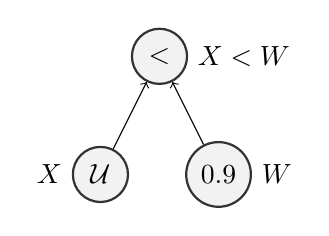
\begin{tikzpicture}[<-]
  \tikzstyle{op}=[circle, minimum size = 7mm, thick, draw =black!80, node distance = 5mm, fill=black!5]

  \node [op,label=right:$X < W$] {$<$}
    child{node [op,label=left:$X$] {$\mathcal{U}$}}
    child{node [op,label=right:$W$] {$0.9$}}
  ;
\end{tikzpicture}
}
\end{center}
%
Much like an expression tree, each node in the Bayesian network corresponds to a value produced by the program.  Unlike an expression tree, however, each node represents a distribution rather than a single value.
This network, for example,
contains three random variables ($X$, $W$, and $X<W$), one for each
expression executed in the program (\code{random.uniform(0,1)}, \code{0.9},
and \code{x < w}). The directed edges represent how these
random variables conditionally depend on one another. For example,
the node for the random variable $X
< W$ has edges from two other nodes: $X$ and $W$.

Because each variable is
dependent \emph{only} on its parents in a Bayesian network, the probability
distributions for each node are defined locally. In our example, the
distribution for the $X < W$ node, a Bernoulli random variable, is:
%
$$\prob{X<W~|~X \sim \mathcal{U}, W=0.9}$$
%
Computing the distribution for $X < W$ requires only the
distributions for its
parents, $X$ and $W$. In this case, both parents are leaves in the Bayesian
network: a uniform distribution and a point-mass distribution.

One way to compute the distribution is to sample it. Sampling the root node
consists of generating a sample at each leaf and then propagating the values
through the graph.
% A sample for any node can be computed based only on the samples of its
% parents.
Since Bayesian networks are acyclic, every node generates
only a single value per sample and the running time of each sample is
bounded.

In this example, we can exploit the Bayesian network formulation
to simplify the graph and compute an exact solution without
sampling. By definition, when $X$ is uniformly distributed,
for any constant $c \in [0,1]$, $\prob{X < c} = c$.  Using this
statistical knowledge, we replace the tree in our example with a
single node representing a Bernoulli distribution with probability
0.9.

% In our example, this optimization collapses the program's entire
% network to a single node. To test the \passert, we know exactly
% $\prob{X < W} = 0.9$, so the assertion succeeds and there is no need
% to sample. In general, more complex programs result in more complex
% Bayesian networks, which even after simplification, will require
% sampling.

% When sampling, we verify \passerts probabilistically with a bounded
% probability of error. A lower error probability generally means higher
% confidence in the verification but more cost to compute. We use
% hypothesis testing to verify a \passert probabilistically based on
% samples.  A hypothesis test requires three parameters: $B$,  a
% Bernoulli distribution to test (i.e., $X < W$); $\alpha$, the
% confidence level; and $u$, such that $\expc{B} >
% u$ at the $\alpha$ confidence level.  The programmer must provide the
% boolean expression to test, which induces $B$, but may use default
% parameters for $\alpha$ and $u$: 0.05 for $\alpha$ and 0.5 for
% $u$, which specifies that $B$ is more
% likely to be true than false with 95\% confidence.  Using a hypothesis
% test bounds the probabilities of both false positives and false
% negatives.  In cases where the necessary number of samples to meet the
% confidence levels is infeasible, the test returns an ``unknown''
% result, meaning that the \passert is neither proven nor disproven.
% Section~\ref{passert:sec:sample} describes the hypothesis testing approach in
% more detail.

% Our verification
% implies that if we ran a program 100 times, we would say \code{B >
%   0.5} when in reality \code{B <= 0.5} at most 5\% of the time.  In
% other words, the confidence interval bounds false-positives.  To bound
% false-negatives, we use an over-approximation of the maximum variance
% in a Bernoulli distribution.


%\paragraph{Summary}
The Bayesian network abstraction for probabilistic programs yields two major
advantages.
First, it gives a probabilistic semantics to programs and \passert
statements.
Appendix~\ref{app:passert} formalizes our probabilistic semantics and proves that
sampling the Bayesian representation is equivalent to sampling the original
program.
Second, we exploit 
probabilistic algebras and statistical properties of random variables to optimize the
verification process. In some cases, we verify \passerts without sampling.
Section~\ref{passert:sec:optim} introduces these 
optimizations.
% Third, we symbolically represent some loops that perform reductions over
% random variables as nodes in our Bayesian network, making them amenable to
% optimizations.  For all other loops, we use sampling to estimate their
% effect. 
% Section~\ref{passert:sec:sample} discusses how we sample loops to probabilistically verify  \passerts and bound
% error in that verification.
% Removing this advantage since it seems unrelated to the Bayesian-network
% formulation. -ALDS


